\subsubsection{Experiment 1}
Table \ref{table:expone} shows an excerpt of the test results.
We see that, as the problem size grows, the \texttt{construct} implementation
becomes faster and faster in comparison with \texttt{all}.
This is likely due to the fact that we save more time for each problem we do
\emph{not} need to solve, as $n$ grows.

A table with results for all $n=100,200,\ldots,2000$ can found in Appendix
\ref{app:exp1}.

\begin{table}[ht!]
    \centering
    \caption{An excerpt of test results from experiment 1.}
\begin{tabular}{lrrr}
    $n$ & \texttt{construct} & \texttt{all} & Percent Faster \\ \hline
    500 & 4.9                & 5.9          & 16.9\% \\
   1000 & 42.1               & 53.0         & 20.6\% \\
   1500 & 181.5              & 234.5        & 22.6\% \\
   2000 & 547.1              & 710.2        & 23.0\%
\end{tabular}
\label{table:expone}
\end{table}

Figure \ref{fig:constructbone} shows the number of seconds used to solve problems
of different sizes $n$, with two different implementations.
The figure shows a plot of 
\begin{figure}[ht!]
    \centering
    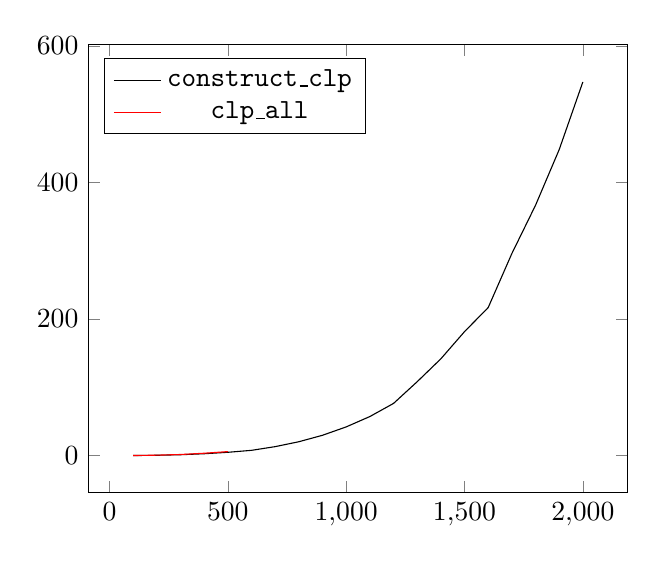
\begin{tikzpicture}
    \begin{axis}[
        legend pos=north west]

        \addplot[black] plot coordinates {
%            (0, 0.000012)
            (100, 0.120660)
            (200, 0.521410)
            (300, 1.307679)
            (400, 2.771161)
            (500, 4.879012)
            (600, 7.744716)
            (700, 13.167763)
            (800, 20.332959)
            (900, 29.800924)
            (1000, 42.052462)
            (1100, 57.228555)
            (1200, 76.425515)
            (1300, 108.207058)
            (1400, 141.722463)
            (1500, 181.548302)
            (1600, 216.743981)
            (1700, 295.849322)
            (1800, 366.523868)
            (1900, 448.033278)
            (2000, 547.087066)
        };

        \addplot[red] plot coordinates {
%            (0, 0.000001)
            (100, 0.155080)
            (200, 0.671939)
            (300, 1.656583)
            (400, 3.510805)
            (500, 5.887408)
        };

        \legend{\texttt{construct\_clp}, \texttt{clp\_all}}
    \end{axis}
\end{tikzpicture}

    \caption{Seconds used to solve all $s(1, n)$ subinstances of randomly
             generated problems of size $n$. The x-axis represents $n$, the
             number of edges in the network, i.e. the number of
             variables/columns in the QP problem. The y-axis represents the
             number of seconds used.}
    \label{fig:constructbone}
\end{figure}
